\documentclass{article}
\usepackage{graphicx}
\usepackage[utf8]{inputenc}
\usepackage[polish]{babel}
\usepackage[T1]{fontenc}
\usepackage{geometry}
\usepackage{longtable}
\usepackage{hyperref}
\usepackage{enumitem}
\usepackage{array}
\usepackage{float}
\newcolumntype{C}[1]{>{\centering\arraybackslash}m{#1}}


\title{Miasta posiadają obiekty zabytkowe. Zabytki podlegają konserwacji przez konserwatorów. }
\author{Karolina Glaza \\ \url{https://github.com/kequel}}
\date{Listopad 2024}

\begin{document}

\maketitle

\section{Opis projektu}
Baza danych służąca do zarządzania konserwacją zabytków, obejmuje informacje o zabytkach, przeglądach technicznych, konserwacjach oraz opiekunach odpowiedzialnych za ich stan. Zawiera dane dotyczące konserwatorów i firm konserwatorskich, którzy wykonują zlecenia konserwacyjne, wraz z raportami z wykonanych prac.   \\

\section{Szczegółowy opis projektu}

\subsection{Klient}
Klientem jest Departament Ochrony Zabytków Ministerstwa Kultury i Dziedzictwa Narodowego. W szczególności osoby odpowiedzialne za planowanie konserwacji - planiści i kierownicy konserwacji. 

\subsection{Cel bazy}
Celem bazy jest utrzymanie historii konserwacji zabytków, informacji o pracach, kosztach, przeglądach technicznych i osobach odpowiedzialnych za konserwacje. Rozwiąże to problemy związane z monitorowaniem stanu zabytków, nadzorem nad pracami konserwatorskimi oraz przekazywaniem informacji o historii konserwacji podwykonawcom. Ułatwi także kontakt z osobami odpowiedzialnymi za zlecenia oraz pozwoli monitorować koszty. 

\subsection{Stanowiska pracy wspomagane przez system}
\begin{itemize}
    \item \textbf{Planiści} - Historia konserwacji pomoże wybrać zabytki do kolejnych prac, dzięki zapisywanym stanom technicznym, ułatwi kontakt z wykwalifikowanymi pod to specjalistami.
    \item \textbf{Księgowi} - Przechowywane w bazie koszty oraz daty poszczególnych konserwacji pozwalają na monitorowanie wydatków oraz łatwe sprawdzenie wszelkich statystyk na ich temat.
    \item \textbf{Konserwatorzy} - Dzięki przechowywaniu historii konserwacji oraz zaleceń od poprzednich zleceniobiorców, prace konserwatorskie mogą być sprawniej organizowane.
\end{itemize}

\subsection{Scenariusze użycia (interakcje z systemem)}
\begin{itemize}
    \item Księgowy: sprawdza wydatki danego roku. 
    \item Konserwator: wprowadza raport z konserwacji, sprawdza stan zlecenia. 
    \item Planiści: planują konserwacje, wprowadzają zlecenia konserwacyjne oraz monitorują prace. 
\end{itemize}

\subsection{Przykładowe zapytania}
\begin{itemize}
    \item Jakie były koszty konserwacji w 2020 roku na zabytki miasta Gdańsk?
    \item Kto jest odpowiedzialny za ostatnią konserwację zamku?
    \item Kto opiekuje się zabytkiem pod danym zleceniem?
    \item W czym specjalizują się konserwatorzy w danej firmie? 
    \item Które zabytki są obecnie w najgorszym stanie technicznym?
    \item Czy dana konserwacja została rozpoczęta o czasie?
\end{itemize}

\subsection{Wykluczenia}
Baza nie będzie zawierała szczegółowych informacji o zasobach firm konserwatorskich ani danych finansowych niezwiązanych bezpośrednio z konserwacją zabytków (np. rozliczeń z konserwatorami). 

\section{ERD Diagram}
\begin{figure}[H]
    \centering
    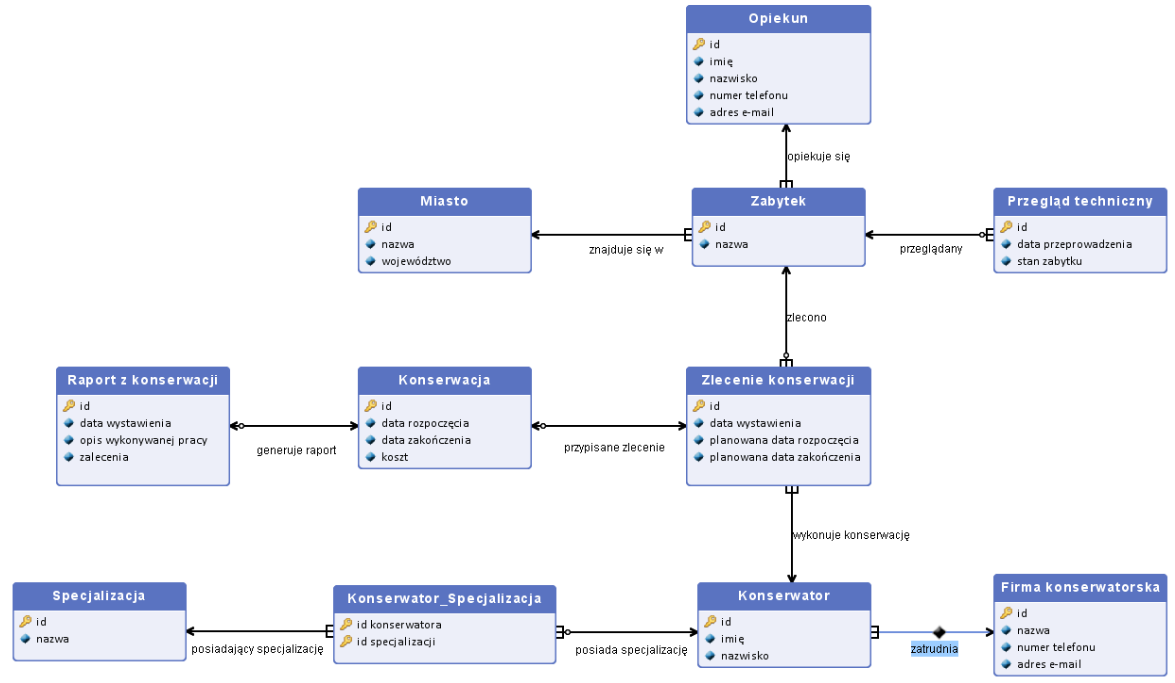
\includegraphics[width=0.8\textwidth]{diagram.png}
    \label{fig:diagram}
\end{figure}

\section{Opis zbioru encji}
\centering
\subsection*{Opiekun}
Przechowuje dane osób odpowiedzialnych za opiekę nad konkretnymi zabytkami. Głównym kluczem identyfikującym jest unikalne id opiekuna. Naturalnym kluczem mógłby być adres e-mail lub numer telefonu. Nowy opiekun trafia do zbioru w momencie przypisania go do zabytku. Pozostaje w zbiorze do momentu, gdy dany opiekun nie jest już przypisany do żadnego zabytku - w przypadku aktualizacji opiekunów.  
\begin{longtable}{|C{3cm}|c|C{4.5cm}|C{5cm}|}
\hline
\textbf{Nazwa} & \textbf{Klucz} & \textbf{Typ/Dziedzina} & \textbf{Opis} \\ \hline
id & Tak & liczba naturalna & identyfikator opiekuna \\ \hline 
imię & Nie & ciąg znaków od 3 do 30 & imię osoby odpowiedzialnej za nadzór nad zabytkiem \\ \hline 
nazwisko & Nie & ciąg znaków od 3 do 30 & nazwisko osoby odpowiedzialnej za nadzór nad zabytkiem \\ \hline 
numer telefonu & Nie & liczba naturalna 11 cyfrowa & kontaktowy numer telefonu do opiekuna \\ \hline
adres e-mail & Nie & ciąg 5-40 znaków zawierający znak "@" i zakończony sekwencją ".com" & kontaktowy adres e-mail do opiekuna \\ \hline
\end{longtable}

\subsection*{Zabytek}
Obejmuje informacje o poszczególnych obiektach zabytkowych, nad którymi sprawowana jest opieka i które mogą wymagać konserwacji. Unikalnym identyfikatorem jest id zabytku. Naturalnym kryterium tożsamości może być unikalna nazwa powszechna zabytku. Zabytek trafia do zbioru w momencie jego uznania jako obiekt zabytkowy. Zabytek nie pozostaje w zbiorze na stałe, usuwany gdy przestaje być uznawany za obiekt zabytkowy.  
\begin{longtable}{|C{3cm}|c|C{4.5cm}|C{5cm}|}
\hline
\textbf{Nazwa} & \textbf{Klucz} & \textbf{Typ/Dziedzina} & \textbf{Opis} \\ \hline
id & Tak & liczba naturalna & identyfikator zabytku \\ \hline
nazwa & Nie & ciąg 3-30 znaków & nazwa powszechna zabytku \\ \hline
\end{longtable}

\subsection*{Przegląd techniczny}
Gromadzi informacje na temat okresowych kontroli stanu technicznego zabytków, w tym datę przeglądu i ocenę stanu. Głównym kluczem jest id przeglądu. Przegląd techniczny jest dodawany do zbioru w momencie jego wykonania. Przeglądy historyczne pozostają w zbiorze na stałe jako dokumentacja stanu zabytku na przestrzeni czasu.  
\begin{longtable}{|C{3cm}|c|C{4.5cm}|C{5cm}|}
\hline
\textbf{Nazwa} & \textbf{Klucz} & \textbf{Typ/Dziedzina} & \textbf{Opis} \\ \hline
id & Tak & liczba naturalna & identyfikator przeglądu technicznego \\ \hline 
data przeprowadzenia & Nie & data z kalendarza gregoriańskiego łącznie z rokiem zapisana w formacie: DD.MM.RRRR  & data przeglądu technicznego określająca moment oceny stanu zabytku  \\ \hline
stan zabytku & Nie & liczba całkowita z przedziału 1-10 & ocena stanu technicznego zabytku w danej skali  \\ \hline
\end{longtable}

\subsection*{Miasto}
Przechowuje informacje o miastach, w których znajdują się zabytki objęte opieką. Kluczem głównym jest unikalne id miasta, naturalnym mogłaby być jego nazwa. Miasto zostaje dodane do zbioru w momencie dodania pierwszego zabytku w tym mieście. Miasta nie pozostają w zbiorze na stałe, jeśli wszystkie zabytki w danym mieście zostaną usunięte z bazy (przestaną być obiektami zabytkowymi), usuwane jest także miasto.  
\begin{longtable}{|C{3cm}|c|C{4.5cm}|C{5cm}|}
\hline
\textbf{Nazwa} & \textbf{Klucz} & \textbf{Typ/Dziedzina} & \textbf{Opis} \\ \hline
id & Tak & liczba naturalna & identyfikator miasta \\ \hline 
nazwa & Nie & ciąg 3-30 znaków & nazwa miasta w którym znajduje się zabytek \\ \hline
województwo & Nie & ciąg 7-19 znaków & nazwa województwa do którego przynależy miasto \\ \hline
\end{longtable}

\subsection*{Zlecenie konserwacji}
Zawiera informacje o zleceniach konserwacji dla zabytków, wraz z datą wystawienia i planowanymi datami rozpoczęcia oraz zakończenia. Głównym kluczem jest unikalne id zlecenia. Zlecenie konserwacji trafia do zbioru w momencie jego wystawienia. Zlecenia pozostają w zbiorze jako dokumentacja konserwacji, chyba że zostaną anulowane (przed rozpoczęciem prac) - są wtedy usuwane.  
\begin{longtable}{|C{3cm}|c|C{4.5cm}|C{5cm}|}
\hline
\textbf{Nazwa} & \textbf{Klucz} & \textbf{Typ/Dziedzina} & \textbf{Opis} \\ \hline
id & Tak & liczba naturalna & identyfikator zlecenia \\ \hline 
data wystawienia & Nie & data z kalendarza gregoriańskiego łącznie z rokiem zapisana w formacie: DD.MM.RRRR  & data określająca moment formalnego zamówienia prac \\ \hline 
planowana data rozpoczęcia & Nie & data z kalendarza gregoriańskiego łącznie z rokiem zapisana w formacie: DD.MM.RRRR  & data określająca zaplanowany moment rozpoczęcia prac \\ \hline
planowana data zakończenia & Nie & data z kalendarza gregoriańskiego łącznie z rokiem zapisana w formacie: DD.MM.RRRR  & data określająca zaplanowany moment zakończenia prac \\ \hline
\end{longtable}

\subsection*{Konserwacja}
Przechowuje informacje o konkretnych działaniach konserwatorskich wykonanych na zabytek, takich jak daty rozpoczęcia, zakończenia i poniesione koszty. Głównym kluczem jest unikalne id konserwacji. Konserwacja jest dodawana do zbioru po rozpoczęciu prac - albo zgodnie ze zleceniem, albo z opóźnieniem. Konserwacje pozostają w zbiorze jako dokumentacja wykonanych prac. Dopóki konserwacja nie jest zakończona - jej atrybut data zakończenia, pozostaje "NULL".  
\begin{longtable}{|C{3cm}|c|C{4.5cm}|C{5cm}|}
\hline
\textbf{Nazwa} & \textbf{Klucz} & \textbf{Typ/Dziedzina} & \textbf{Opis} \\ \hline
id & Tak & liczba naturalna & identyfikator konserwacji \\ \hline 
data rozpoczęcia & Nie & data z kalendarza gregoriańskiego łącznie z rokiem zapisana w formacie: DD.MM.RRRR & data określająca moment rozpoczęcia prac \\ \hline 
data zakończenia & Nie & data z kalendarza gregoriańskiego łącznie z rokiem zapisana w formacie: DD.MM.RRRR lub NULL & data określająca moment zakończenia prac, ewentualnie jej brak sygnalizowany przez "NULL" \\ \hline
koszt & Nie & liczba dodatnia z maksymalnie dwoma cyframi po przecinku, domyślnie wyrażona w polskich złotówkach & całkowity koszt konserwacji \\ \hline
\end{longtable}

\subsection*{Raport z konserwacji}
Obejmuje raporty z wykonanych prac konserwacyjnych, w tym opis działań i zalecenia dotyczące dalszej opieki. Kluczem głównym jest unikalne id raportu. Raport jest dodawany do zbioru po zakończeniu konserwacji. Raporty pozostają w zbiorze jako dokumentacja prac konserwacyjnych, bez usunięcia w przyszłości.   
\begin{longtable}{|C{3cm}|c|C{4.5cm}|C{5cm}|}
\hline
\textbf{Nazwa} & \textbf{Klucz} & \textbf{Typ/Dziedzina} & \textbf{Opis} \\ \hline
id & Tak & liczba naturalna & identyfikator raportu \\ \hline 
data wystawienia & Nie & data z kalendarza gregoriańskiego łącznie z rokiem zapisana w formacie: DD.MM.RRRR  & data określająca moment wystawienia raportu \\ \hline 
opis wykonywanej pracy & Nie & ciąg do 300 znaków & opis prac konserwacyjnych które zostały wykonane \\ \hline
zalecenia & Nie & ciąg do 300 znaków & zalecenia od konserwatora dla opiekunów oraz przyszłych konserwatorów zabytku dotyczące dalszych działań lub utrzymania zabytku \\ \hline
\end{longtable}

\subsection*{Konserwator}
Przechowuje informacje o osobach zatrudnionych jako konserwatorzy. Kluczem głównym jest unikalne id konserwatora. Konserwator jest dodawany do zbioru w momencie zatrudnienia do wykonania jakiejś konserwacji. Dane konserwatora pozostają w zbiorze, nawet jeśli zakończy pracę, by służyć do potencjalnego sprawdzania historii konserwatorów zabytku.
\begin{longtable}{|C{3cm}|c|C{4.5cm}|C{5cm}|}
\hline
\textbf{Nazwa} & \textbf{Klucz} & \textbf{Typ/Dziedzina} & \textbf{Opis} \\ \hline
id & Tak & liczba naturalna & identyfikator konserwatora \\ \hline 
imię & Nie & ciąg 3-30 znaków & imię osoby odpowiedzialnej za prace konserwacyjne \\ \hline
nazwisko & Nie & ciąg 3-30 znaków & nazwisko osoby odpowiedzialnej za prace konserwacyjne \\ \hline
\end{longtable}

\subsection*{Firma konserwatorska}
Przechowuje dane firm oferujących usługi konserwatorskie, które zatrudniają konserwatorów. Głównym kluczem jest unikalne id firmy konserwatorskiej. Naturalnym kryterium tożsamości mogłaby być formalna nazwa firmy. Firma konserwatorska trafia do zbioru w momencie, gdy jakiś jej konserwator przeprowadza konserwacje dla instytucji. Firma pozostaje w zbiorze na stałe.  
\begin{longtable}{|C{3cm}|c|C{4.5cm}|C{5cm}|}
\hline
\textbf{Nazwa} & \textbf{Klucz} & \textbf{Typ/Dziedzina} & \textbf{Opis} \\ \hline
id & Tak & liczba naturalna & identyfikator firmy konserwatorskiej \\ \hline 
nazwa & Nie & ciąg 1-30 znaków & pełna formalna nazwa firmy zajmującej się pracami konserwatorskimi \\ \hline 
numer telefonu & Nie & liczba naturalna 11 cyfrowa & kontaktowy numer telefonu do firmy \\ \hline
adres e-mail & Nie & ciąg 5-40 znaków zawierający znak "@" i zakończony sekwencją ".com" & kontaktowy adres mailowy firmy \\ \hline
\end{longtable}

\subsection*{Konserwator\_Specjalizacja}
Tabela pośrednia dla relacji "wiele do wielu", która przechowuje przypisania specjalizacji do konserwatorów. Kluczem głównym jest kombinacja id konserwatora i id specjalizacji, co jednoznacznie określa, jaką specjalizację posiada dany konserwator. Przypisanie specjalizacji do konserwatora trafia do zbioru w momencie, gdy konserwator uzyska odpowiednią kwalifikację w danej specjalizacji konserwatorskiej. Konserwator nie traci swoich umiejętności, pozostaje więc w bazie na stałe.  
\begin{longtable}{|C{3cm}|c|C{4.5cm}|C{5cm}|}
\hline
\textbf{Nazwa} & \textbf{Klucz} & \textbf{Typ/Dziedzina} & \textbf{Opis} \\ \hline
id konserwatora & Tak & liczba naturalna & identyfikator konserwatora posiadającego specjalizację \\ \hline
id specjalizacji & Tak & liczba naturalna & identyfikator specjalizacji posiadanej przez konserwatora \\ \hline
\end{longtable}

\subsection*{Specjalizacja}
Rodzaje specjalizacji, które mogą być przypisane konserwatorom, określające ich zakres kompetencji. Głównym kluczem jest unikalne id specjalizacji. Naturalnym kryterium tożsamości może być nazwa specjalizacji. Specjalizacja trafia do bazy gdy dodawany jest jakiś konserwator, który ją posiada. Specjalizacje pozostają w zbiorze na stałe, by podobnie jak konserwatorzy służyć do potencjalnego sprawdzania historii konserwatorów zabytku.  
\begin{longtable}{|C{3cm}|c|C{4.5cm}|C{5cm}|}
\hline
\textbf{Nazwa} & \textbf{Klucz} & \textbf{Typ/Dziedzina} & \textbf{Opis} \\ \hline
id & Tak & liczba naturalna & identyfikator specjalizacji \\ \hline
nazwa & Nie & ciąg 3-30 znaków & nazwa specjalizacji, opisująca obszar wiedzy konserwatora \\ \hline
\end{longtable}

\end{document}
